\documentclass[10pt]{beamer}
\usepackage[utf8]{inputenc}
\usepackage{xeCJK}
\usepackage{graphicx}
\usepackage {mathtools}
\usepackage{utopia} %font utopia imported
\usetheme{CambridgeUS}
\usecolortheme{dolphin}

% Russian language
\usepackage[russian]{babel}
\usepackage[utf8]{inputenc}
\usepackage[T2A, T1]{fontenc}
\usepackage{fontspec}
\usefonttheme{serif}
\setmainfont{Times New Roman}

% set colors
\definecolor{myNewColorA}{RGB}{126,12,110}
\definecolor{myNewColorB}{RGB}{165,85,154}
\definecolor{myNewColorC}{RGB}{203,158,197}
\setbeamercolor*{palette primary}{bg=myNewColorC}
\setbeamercolor*{palette secondary}{bg=myNewColorB, fg = white}
\setbeamercolor*{palette tertiary}{bg=myNewColorA, fg = white}
\setbeamercolor*{titlelike}{fg=myNewColorA}
\setbeamercolor*{title}{bg=myNewColorA, fg = white}
\setbeamercolor*{item}{fg=myNewColorA}
\setbeamercolor*{caption name}{fg=myNewColorA}
\usefonttheme{professionalfonts}
\usepackage{natbib}
\usepackage{hyperref}
%------------------------------------------------------------
%\titlegraphic{\includegraphics[height=1.5cm]{nku-logo.eps}}

\setbeamerfont{title}{size=\large}
\setbeamerfont{subtitle}{size=\small}
\setbeamerfont{author}{size=\small}
\setbeamerfont{date}{size=\small}
\setbeamerfont{institute}{size=\small}
\title[On the problem of repeated supervised learning]{On the problem of repeated supervised learning}
\subtitle{My first scientific paper}
\author[Andrey Veprikov]{Andrey Veprikov \and Anton Khritankov
\and Alexander Afanasyev}

\institute[veprikov.as@phystech.edu]{
MIPT\\
Dolgoprudny, Russia}

\date[Spring 2023]
{Spring 2023}

%------------------------------------------------------------
%This block of commands puts the table of contents at the 
%beginning of each section and highlights the current section:
%\AtBeginSection[]
%{
%  \begin{frame}
%    \frametitle{Contents}
%    \tableofcontents[currentsection]
%  \end{frame}
%}
%\AtBeginSection[]{
%  \begin{frame}
%  \vfill
%  \centering
%  \begin{beamercolorbox}[sep=8pt,center,shadow=true,rounded=true]{title}
%    \usebeamerfont{title}\insertsectionhead\par%
%  \end{beamercolorbox}
%  \vfill
%  \end{frame}
%}
%------------------------------------------------------------

\begin{document}

%The next statement creates the title page.
\frame{\titlepage}
%\begin{frame}
%\frametitle{Содержание}
%\tableofcontents
%\end{frame}
%------------------------------------------------------------
\section{Goals and contributions of paper}
    \begin{frame}{Introduction and Related work}

        In this research paper, we delve into the intricacies of continuous learning artificial intelligence systems as they interact with and influence their environment. 

        Repeated supervised learning appears in many machine learning applications, for example in 
        
        \begin{enumerate}
            \item recommendation systems \cite{khritankov2021existence}
    
            \item healthcare \cite{adam2020hidden}
    
            \item predictive policing \cite{ensign2018runaway}
        \end{enumerate}
        
        Contributions of this paper are as follows
        
        \begin{enumerate}
            \item Develop a mathematical model to examine the process of repeated and multiple learning, prediction, and dataset updating.
    
            \item Find necessary and sufficient conditions for various effects associated with repeated machine learning that can be tested in experiments
    
            \item Conduct several synthetic experiments based on our findings, hoping to contribute to a better understanding of the behavior of continuous learning AI systems.
        \end{enumerate}
        
    \end{frame}

    \begin{frame}{Problem statement}
        The object of our research will be the set $\mathbf{R}$ of distribution density functions
    
        \begin{equation*}
            \mathbf{R} := \left\{f : \mathbb{R}^n \rightarrow \mathbb{R}_+ ~\text{and}~ \int\limits_{\mathbb{R}^n}f(x)dx = 1\right\}
        \end{equation*}
    
        and a mapping $\text{D}$ as feedback loop mapping.

        We consider an autonomous (time-independent explicitly) discrete dynamical system. There is a dedicated variable - the step number, which increases, at step $t$ and $t+1$ of which the ratio is fulfilled

        \begin{equation*}
            f_{t+1}(x) = \text{D}(f_t)(x), \quad \text{for}~ \forall x \in \mathbb{R}^n,
        \end{equation*}
    
        where $\text{D}$ becomes an evolution operator on the space of the specified functions $f$ and the initial function $f_0(x)$ is known.

        According to Conjecture 1 from \cite{khritankov2021hidden} the positive feedback loop in a system $\text{D} : R \rightarrow R$ exists if $\text{D}$ is a contraction mapping, but this conjecture was not proved.
        
    \end{frame}

\section{Main results}
    \begin{frame}{Assumptions for $\text{D}: \mathbf{R} \to \mathbf{R}$}
        \large{\textcolor{myNewColorA}{\textbf{Theorem 1}}}
        \normalsize
    
        If $\|\text{D}\|_1 = 1, \forall f \in \mathbf{R} \hookrightarrow \text{D}(f)(x) \geq 0$ for almost every $x \in \mathbb{R}^n$, and exists $\text{D}^{-1}$ such that $\|\text{D}^{-1}\|_1 \leq 1$, then $\text{D} : \mathbf{R} \to \mathbf{R}$.\\
        
        \large{\textcolor{myNewColorA}{\textbf{Discussion}}}
        \normalsize
        
        In experiments it often difficult to calculate $\text{D}^{-1}$ and especially it's norm, so we make a different assumptions. Distribution of our data is approximating by empirical distribution function \cite{dvoretzky1956asymptotic} as follows (for $n=1$):
        
        \begin{equation*}
            \hat{F}_N(x) := \dfrac{\text{number of elements in sample} \leq x}{N} = \dfrac{1}{N}\sum\limits_{i=1}^N \textbf{1}_{X_i \leq x},
        \end{equation*}
        
        where $X_i$ are elements of sample. We assume that $(X_1, X_2, X_3, ... , X_N)$ are i.i.d. real random variables.
        
        In this case operator $\text{D}$ transoms our data, i.e. translates one empirical distribution function to another. So $\text{D} : \mathbf{R} \to \mathbf{R}$ by constructing our experiment.

    \end{frame}

    \begin{frame}{Inequality on $\|\text{D}\|_q$}
        \large{\textcolor{myNewColorA}{\textbf{Theorem 2}}}
        \normalsize
        
        Consider 
        \begin{equation*}
            f_A(x) = \dfrac{1}{\lambda(A)} \cdot \textbf{1}_{A}(x),
        \end{equation*}

        where $A \subset \mathbb{R}^n$ is arbitrary set of a non-path measure, $\lambda(A)$ -- the measure of a set $A$.

        Then for all $A \subset \mathbb{R}^n :  0 < \lambda(A) < +\infty$ and for all $1 \leq q \leq +\infty$ such that $\text{D}(f_A) \in L_q(\mathbb{R}^n)$ is fulfilled that  

        \begin{equation*}
            \|\text{D}\|_q \geq \int\limits_{A} \text{D}(f_A)(x)dx
        \end{equation*}

        \large{\textcolor{myNewColorA}{\textbf{Discussion}}}
        \normalsize

        To begin with, note that the result of this Theorem does not depend in any way on whether $\text{D}$ converts $\mathbf{R}$ to $\mathbf{R}$.
    
        If you look at it from a probabilistic point of view, then $f_A$ is a distribution density function of vectors uniformly distributed on a set $A$. If $\|\text{D}\|_q \geq 1$, then $\text{D}$ wouldn't be a contraction mapping in $\|\cdot\|_q$, because there always would be function $f \in \mathbf{R}$ such that $\|\text{D}(f)\|_q \geq \|f\|_q$.
        
    \end{frame}

    \begin{frame}{Limit in a weak sense to $\delta$ function}
        \normalsize{\textcolor{myNewColorA}{\textbf{Theorem 3}}}
        \small

        If $f_t : \mathbb{R} \to \mathbb{R}$ such that $\forall t \in \mathbb{N} \hookrightarrow  \|f_t\|_1 = 1$, $f_t(x) \geq 0$ in almost every point $x \in \mathbb{R}$ and
        \begin{equation*}
            \exists \psi : \mathbb{N} \to \mathbb{R} : \psi(t) \underset{t \to +\infty}{\longrightarrow} +\infty ~\text{ and }~
            \exists g \in L_1(\mathbb{R}) ~\text{ such that }~
        \end{equation*}
        \begin{equation*}
            \forall t \in \mathbb{N} ~\forall y \in \mathbb{R} \hookrightarrow f_t\left(\dfrac{y}{\psi(t)}\right) \leq \psi(t) \cdot |g(y)|
        \end{equation*}

        Then $f_t(x) \underset{t \to \infty}{\longrightarrow} \delta(x)$ in a weak sense, i.e.

        \begin{equation*}
            \underset{t \to +\infty}{\lim}\left( \text{ } \int\limits_{-\infty}^{+\infty} f_t(x) \phi(x) dx \text{ } \right) = \phi(0),
        \end{equation*}

        where $\phi$ is continuous function with compact support

        \normalsize{\textcolor{myNewColorA}{\textbf{Discussion}}}
        \small

        If in some step $t$ the model $H(x, \theta, t)$ starts to give good predictions , then, in the probabilistic formulation, this means that the density function of the distribution of the object-sign vectors becomes similar to the delta function. Based on these considerations, we can compare each operator $\text{D}$ to an operator $\widetilde{\text{D}}$, where $\widetilde{\text{D}}$ transforms $\|\mathbf{y} - \mathbf{y_{\text{pred}}}\|$ at each step, where $\mathbf{y_{\text{pred}}} = H(\mathbf{X}, \theta, t)$.
        
    \end{frame}

    \begin{frame}{Consequences of the Theorem 3}
        \normalsize{\textcolor{myNewColorA}{\textbf{Lemma 1}}}
        \small

        If 
            $\forall x \neq 0 \hookrightarrow f_t(x) \underset{t \to \infty}{\longrightarrow} 0$ and $f_t(0) \underset{t \to \infty}{\longrightarrow} +\infty$,
        then we can take
            $\psi(t) = \dfrac{f_t(0)}{|g(0)|}$

        In the following we assume that the operator $\text{D}$  has the form  

        \begin{equation}
            \label{tmp}
            \text{D}^t(f_0)(x) = \psi(t) \cdot f_0(\psi(t) x)
        \end{equation}

        \normalsize{\textcolor{myNewColorA}{\textbf{Lemma 2}}}
        \small

        $\{\text{D}^t\}_{t \in \mathbb{N}}$ is semigroup, i.e. $\text{D}^{\tau} \circ \text{D}^{\kappa} = \text{D}^{\tau + \kappa}$, if and only if $\psi(\tau + \kappa) = \psi(\tau) \cdot \psi(\kappa)$

        \normalsize{\textcolor{myNewColorA}{\textbf{Lemma 3}}}
        \small

        If $\text{D}$ has the form \eqref{tmp}, then \text{D} becomes an isometry in the Kullback–Leibler divergence, i.e. $\forall f_1, f_2 \in \mathbf{R} \hookrightarrow \rho(f_1, f_2) = \rho(\text{D}(f_1), \text{D}(f_2))$

        \normalsize{\textcolor{myNewColorA}{\textbf{Lemma 4}}}
        \small

        If $\text{D}$ has the form \eqref{tmp}, then $\|\{\nu_k^t\}_0^{+\infty} - e_0\|_1 \underset{t \to \infty}{\longrightarrow} 0$, where $\nu_k^t$ -- $k$-th moments of a random variable $\|\mathbf{y} - \mathbf{y_{\text{pred}}}\|$ on step $t$ and $e_0 = (1, 0, 0, 0, ....)$

        \normalsize{\textcolor{myNewColorA}{\textbf{Lemma 5}}}
        \small

        If $\text{D}$ has the form \eqref{tmp} and we consider a set $\mathbf{R^*} := \left\{\left. \phi(s) := \int\limits_{-\infty}^{+\infty} e^{isx} f(x) dx ~\right|~ f \in \mathbf{R} \right\}$ -- set of characteristic functions. Then for all $\phi_0 \in \mathbf{R^*}$ is fulfilled that $\text{D}^t(\phi_0)(s) \underset{t \to \infty}{\longrightarrow} \phi_{\delta}(s) = 1 ~\forall s \in \mathbb{R}$
    \end{frame}

    \begin{frame}{Important example of $\psi$ and $g$}
        \small
        Important example of operator $\text{D}$ that translates any function from $\mathbf{R}$ into a $\delta$ function is as follows

        \begin{equation*}
            \text{D}^t(f_0)(x) = t \cdot f_0(t \cdot x)
        \end{equation*}

        Here we take $g(x) = f_0(x)$ and $\psi(t) = t$. 

        \begin{figure}[h!]
            \centering
            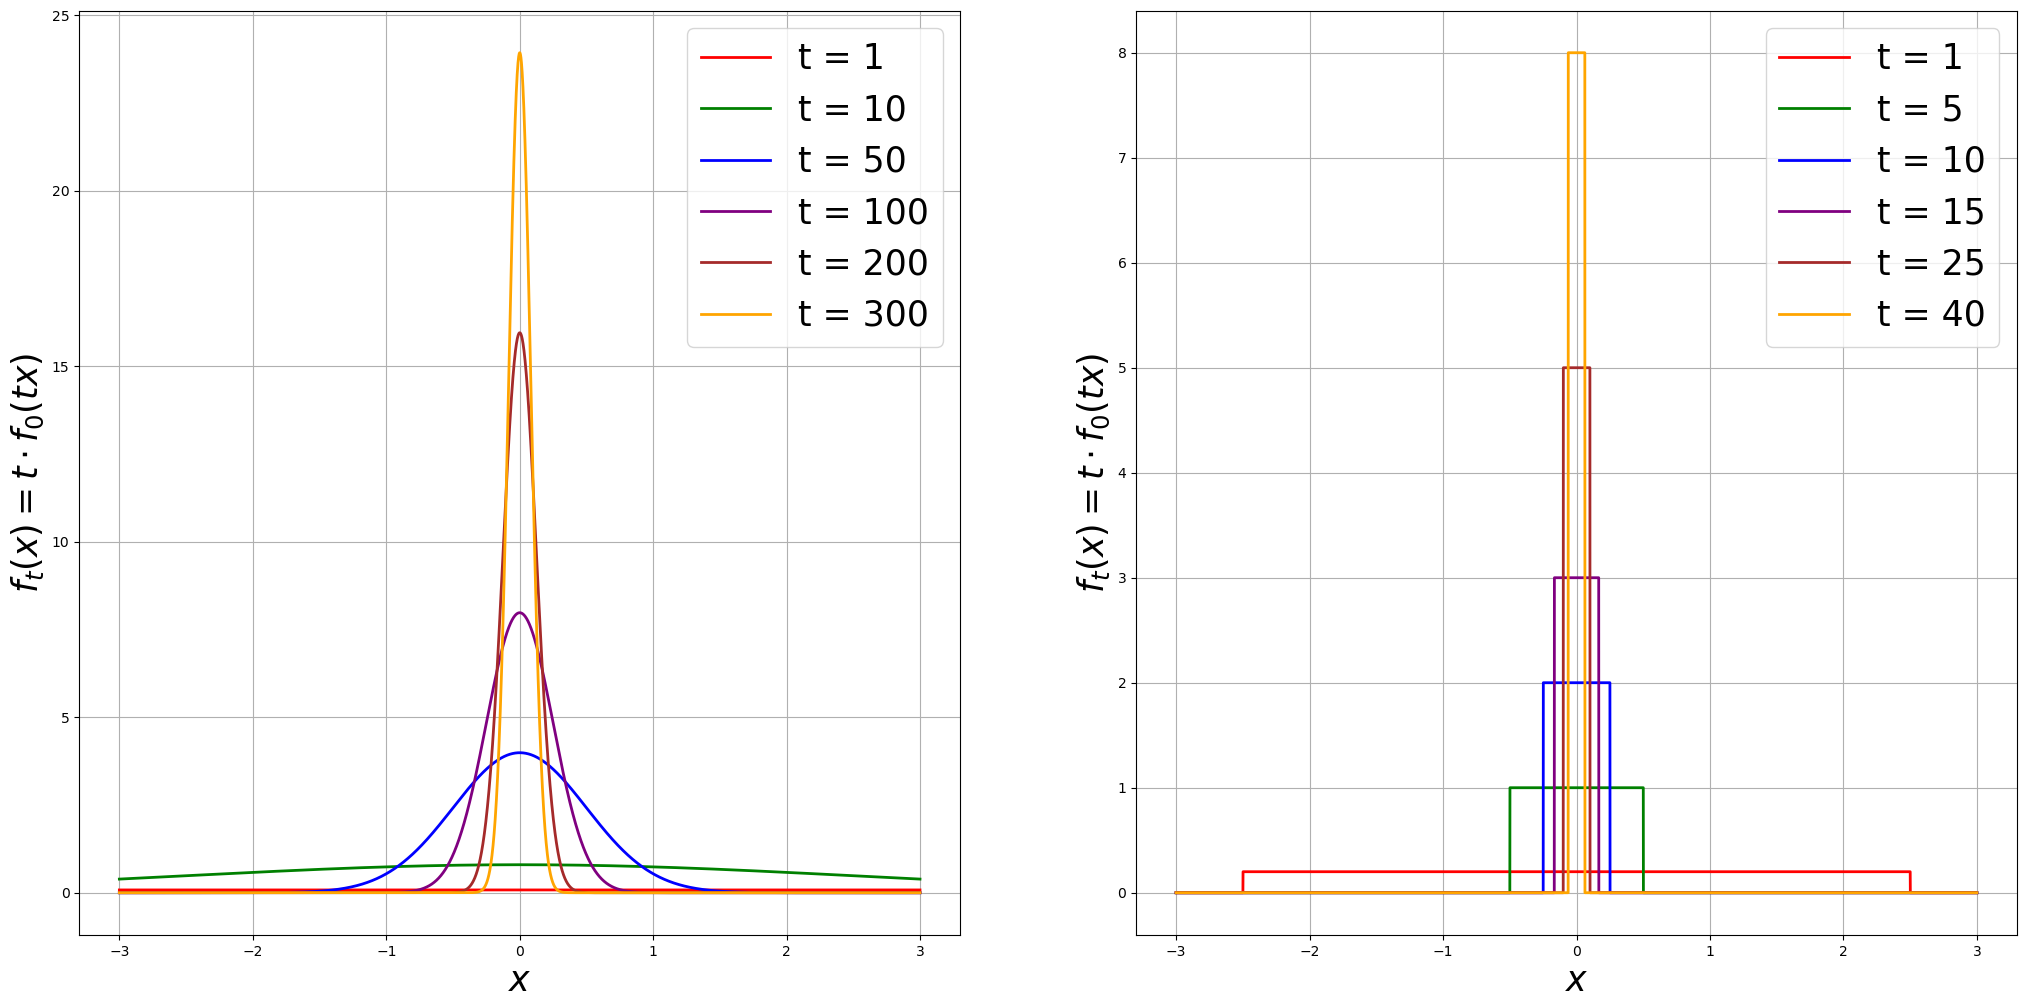
\includegraphics[scale = 0.19]{pictures/example1.png}
            
            Illustration of weak limit to $\delta$ function. $\mathcal{N}(0, 5)$ left, $\mathcal{U}[-2.5, 2.5]$ right.
            \label{example1_fig}
        \end{figure}
        
    \end{frame}

\section{Experiments}

    \begin{frame}{Experiment Design}
        \small
        In this paper we consider linear model, that is solved as Ridge regression with mean squared error loss function. In the formulation of our experiment, we consider $\mathbf{R}$ as space of density functions of random vectors $(\mathbf{x^i}, y_i)$, where $\mathbf{x^i} \in \textbf{X}$ and $y_i \in \textbf{y}$ -- the features and target variable of the $i$-th object.

        \begin{figure}[h!]
            \centering
            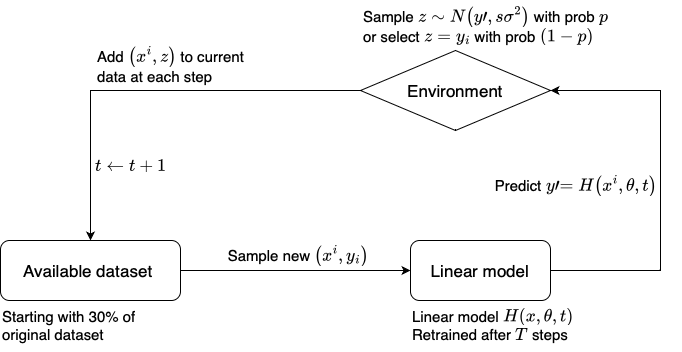
\includegraphics[scale = 0.43]{pictures/Experiment_setup.png}
            
            Experiment setup.
            \label{ex_set}
        \end{figure}

        
    \end{frame}

    \begin{frame}{Dispersion decrease}
        \small
        We measured the standard deviation of $\mathbf{y} - \mathbf{y_{\text{pred}}}$ at different \textit{usage} -- the probability with which we take $(\mathbf{x^i}, z_i)$ into the active dataset and \textit{adherence} -- the parameter by which we multiply $\sigma^2$ when sampling $z_i$.

        \begin{figure}[h!]
            \centering
            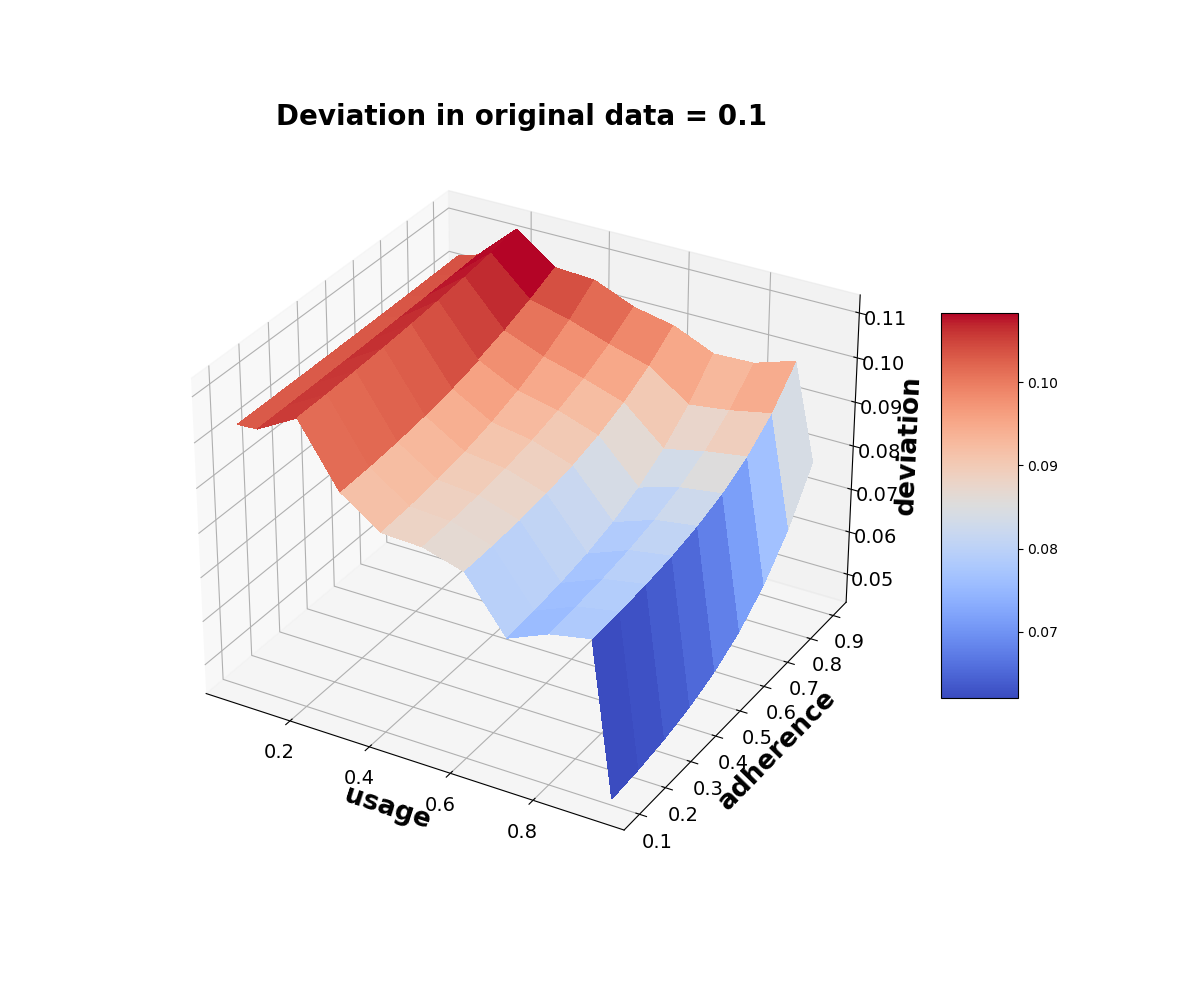
\includegraphics[width=0.325\linewidth]{pictures/3D_plot_0.1.png}
            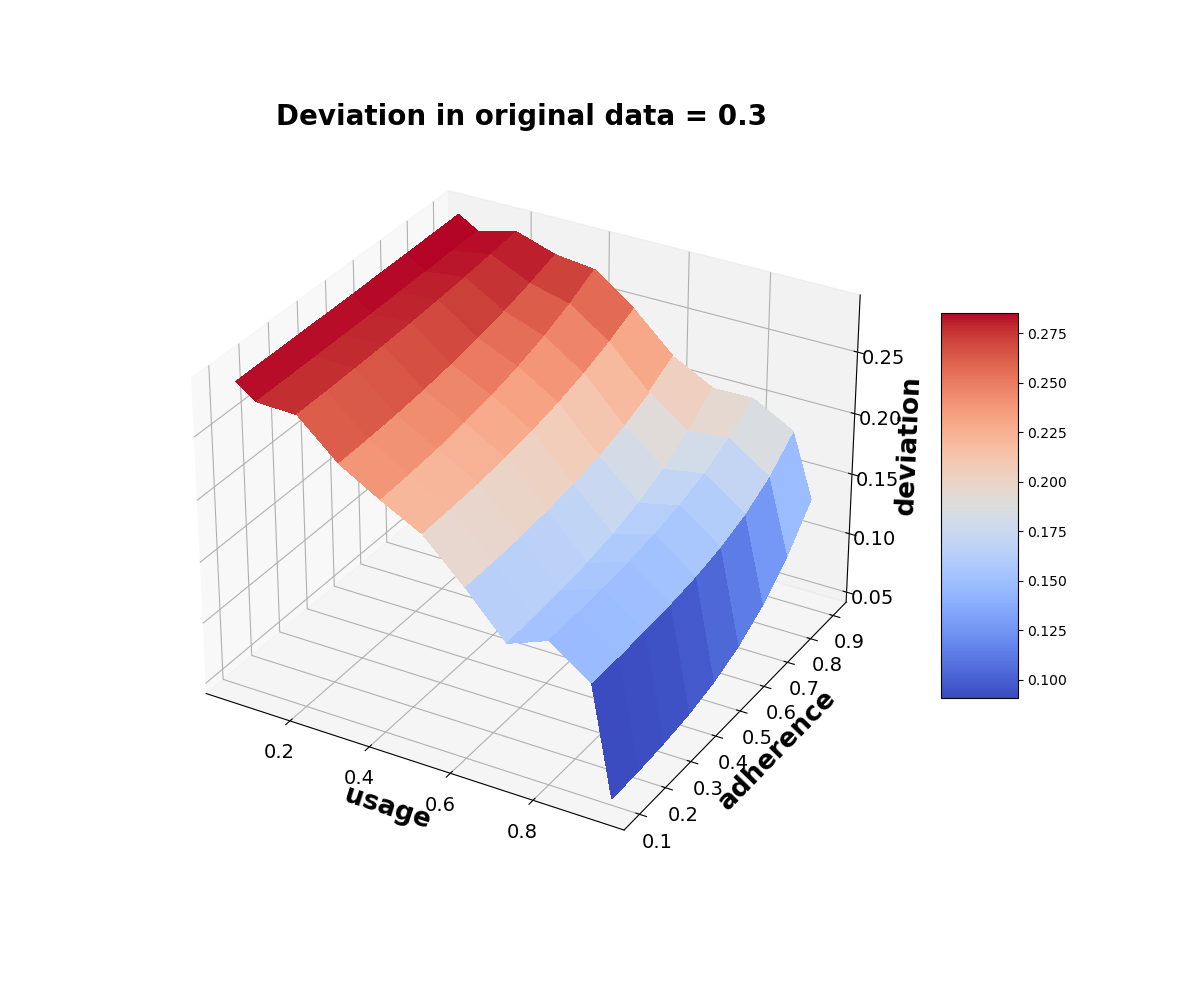
\includegraphics[width=0.325\linewidth]{pictures/3D_plot_0.3.png}
            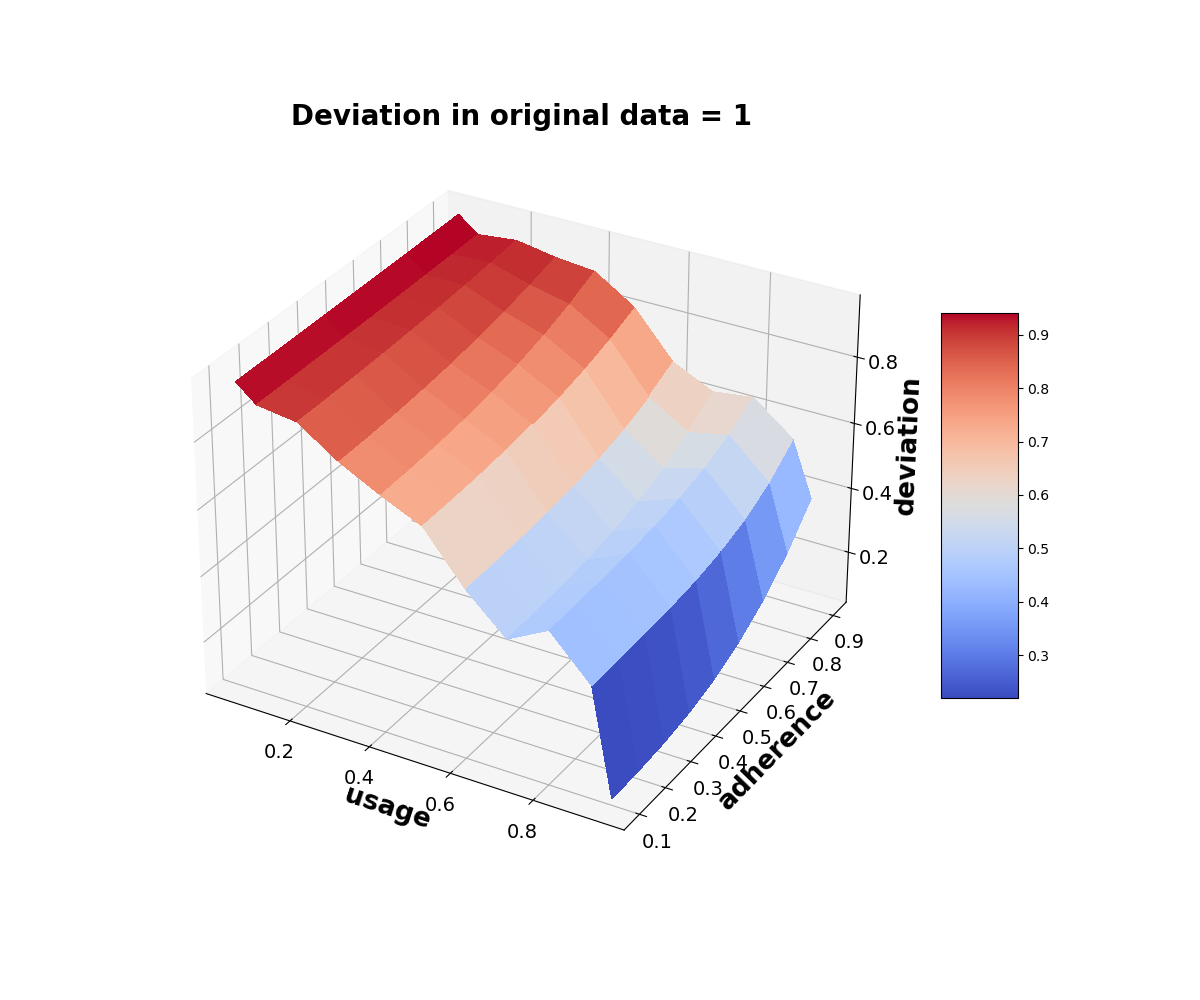
\includegraphics[width=0.325\linewidth]{pictures/3D_plot_1.png}
            
            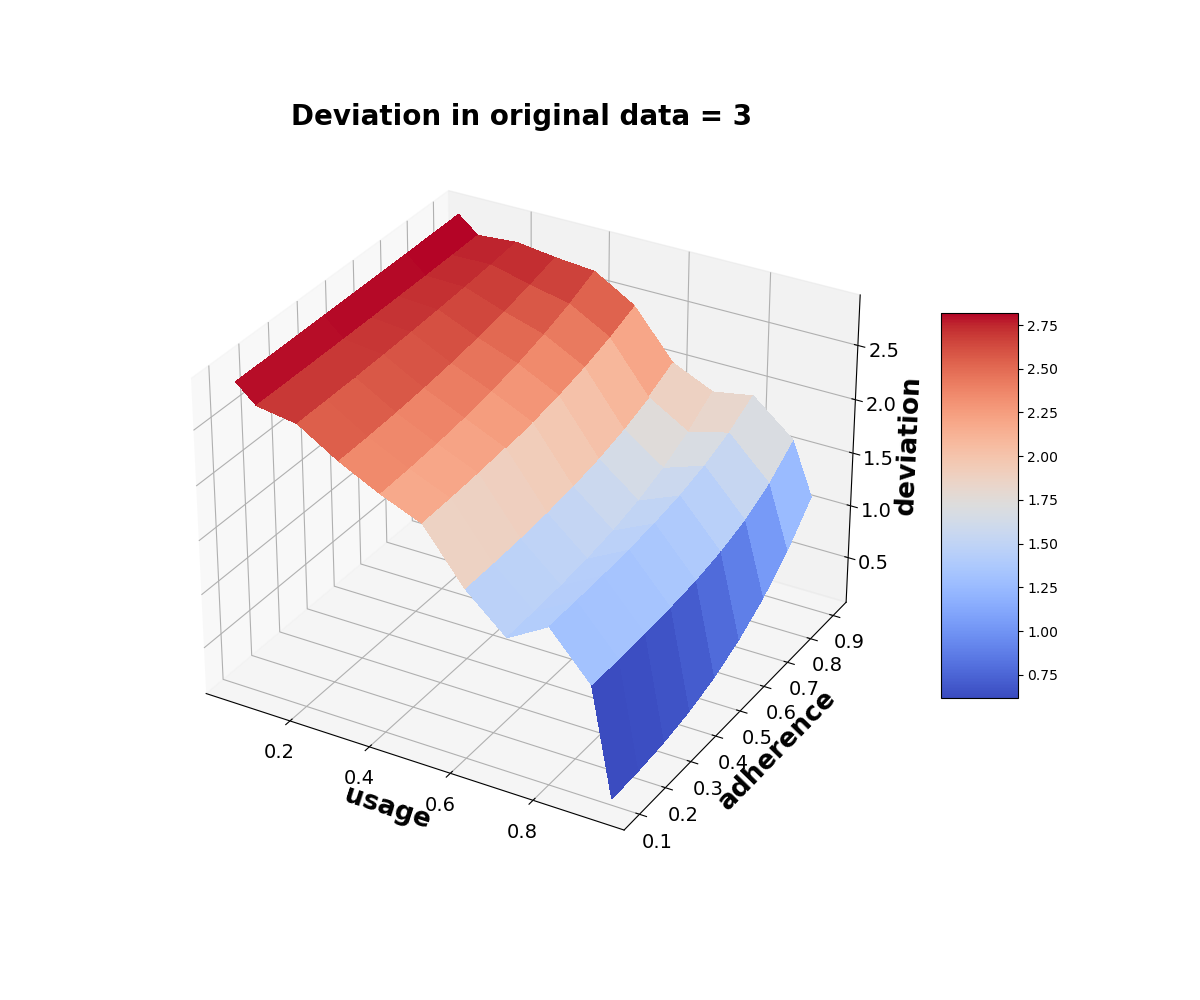
\includegraphics[width=0.33\linewidth]{pictures/3D_plot_3.png}
            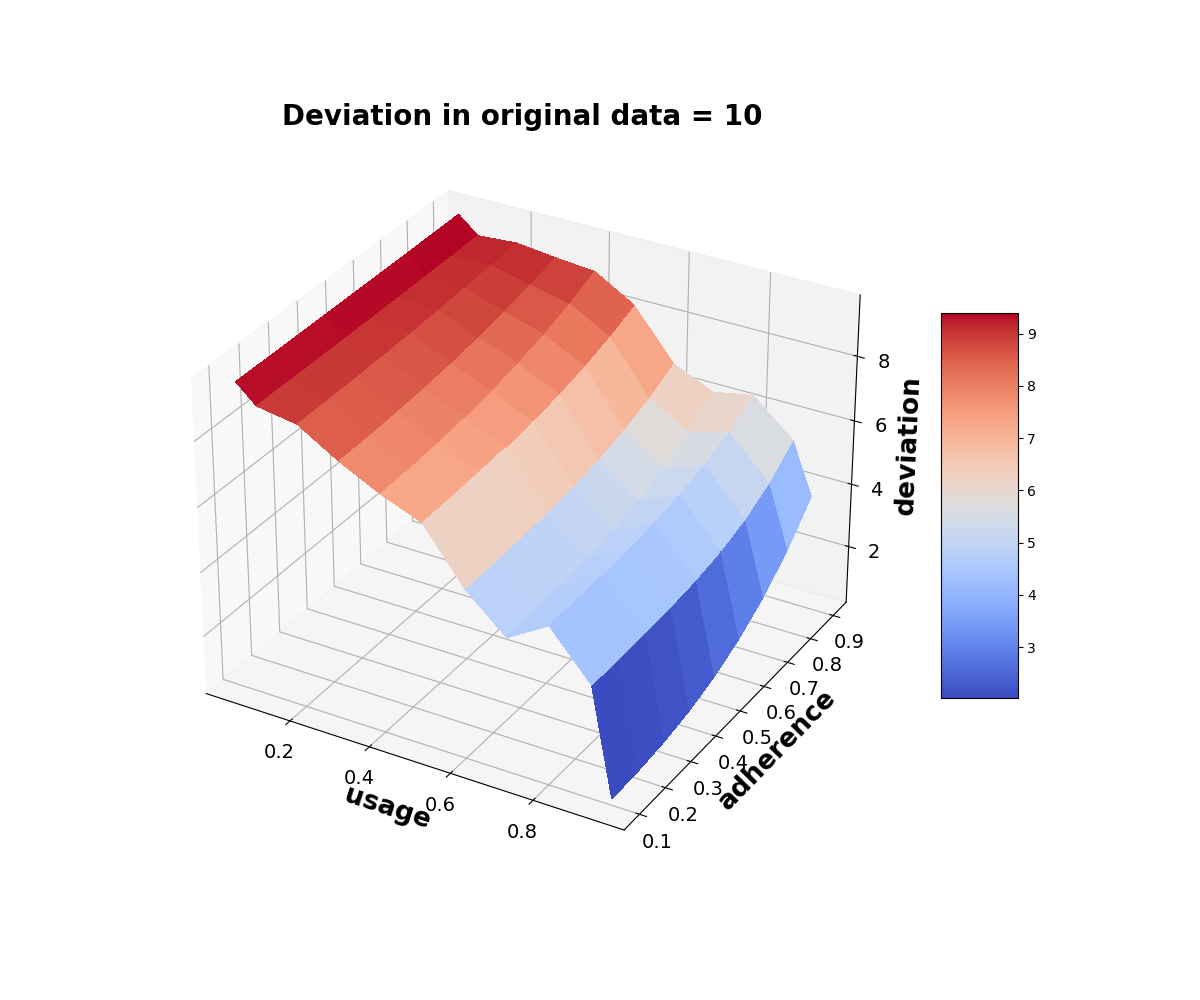
\includegraphics[width=0.33\linewidth]{pictures/3D_plot_10.png}
            
            \caption{3D Graphics for different  noise in original data}
            \label{3D}
        \end{figure}
    \end{frame}

\section{Conclusion}

    \begin{frame}{Conclusion}
        \begin{enumerate}
            \item In this paper we develop a mathematical model to examine the process of repeated learning.

            \item We provide several Theorems and Lemmas based on our mathematical model for better understanding how multiple learning can improve our models.

            \item We conduct some synthetic experiments based on our findings, in which we tested the significance of our theoretical results.
        \end{enumerate}
    \end{frame}





\section{References}
    \begin{frame}{References}
        \footnotesize
        \bibliographystyle{plain}
        \bibliography{refs}  
    \end{frame} 

\end{document}
